\section{Part A - Pre Design Stage}
\subsection{Q1}
In this part, we are asked to calculate the rated torque of the motor.

\begin{equation}
    T_{rated} = \dfrac{P_{nominal}}{\omega_{nominal}} = \dfrac{400kW}{50\pi} = 2546 \; Nm
\end{equation}

\subsection{Q2}
In this part, we are going to calculate the rated frequency of the machine, and depending on the maximum frequency, we will choose a switching frequency.

\begin{equation}
    f_{m,max} = \dfrac{2250}{60} = 37.5 Hz,
\end{equation}

\begin{equation}
    f_{max} = f_{m,max} pp = 75 Hz
\end{equation}

As we increase the switching frequency, the losses will increase. So, we need to choose an adequate switching frequency. Also, to eliminate the lower harmonics we are going to choose a large switching frequency.

We choose the switching frequency as

\begin{equation}
    f_s = 3000
\end{equation}

\subsection{Q3}

We know that DC voltage of a three phase full wave rectifier is:

\begin{equation}
    V_{DC} = 1.35 V_{L-L}
\end{equation}

% DC link design, its simulation results
Therefore, 540V is obtained with the three phase full wave diode rectifier. In order to design a reasonable DC link capacitor, the peak current which is 1700A is considered, and machine is represented with a 0.317 ohm resistor. Desired voltage ripple is decided, and required capacitance value is found from the following schematic.

\begin{center}
\begin{figure}[H]
\centering
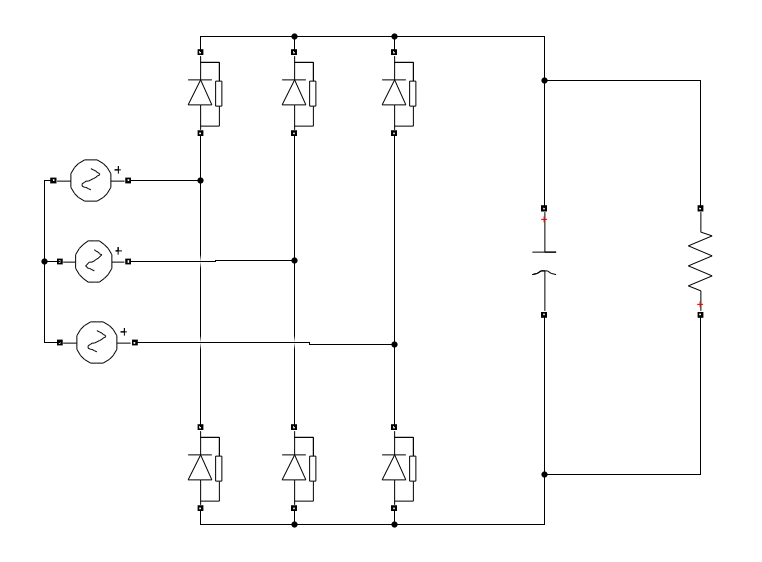
\includegraphics [width= 10 cm]{figs/dclinkschematic.png}
\caption{Circuit Schematic with Representative Resistor}
\label{fig: LABEL}
\end{figure}
\end{center}

For such a system, it is appropriate to have nearly 6\% voltage ripple. From simulations shown in Fig. \ref{fig: dclink}, it is obvious that nearly 5.8\% voltage ripple is obtained with 100 mF capacitor. 

\begin{figure}[H]
        \centering
        \begin{subfigure}[b]{0.475\textwidth}
            \centering
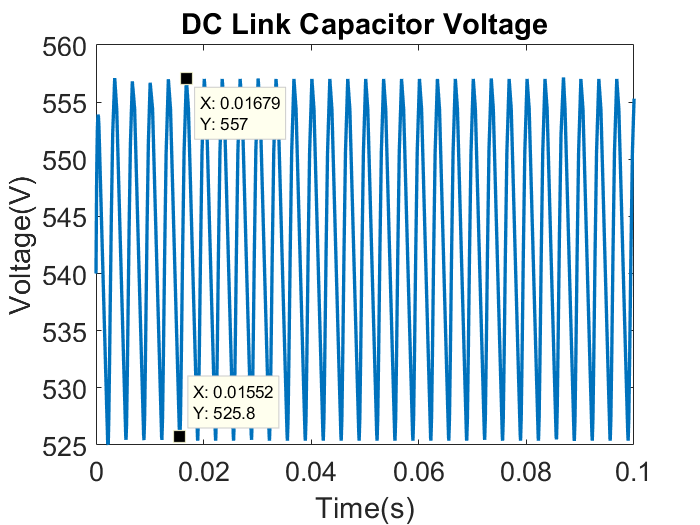
\includegraphics [width= 8 cm]{figs/dclinkvoltage.png}
\caption{DC Link Capacitor Voltage with Resistive Load}
\label{fig: dclink}
        \end{subfigure}
        \hfill
        \begin{subfigure}[b]{0.475\textwidth}  
          \centering
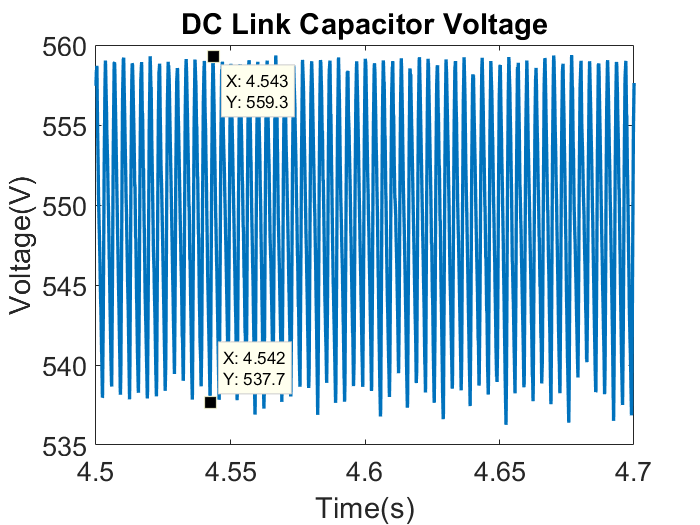
\includegraphics [width= 8cm]{figs/dclinkvoltage_spvm.png}
\caption{DC Link Capacitor Voltage $f_s = 3kHz$}
\label{fig: dclink_spwm}
        \end{subfigure}
        \caption{DC Link voltage for Resistive Load (a) and SPWM (b)}
        \label{fig:b4}
        \end{figure}  

With an inverter, it is known that voltage ripple decreases due to switching frequency. In other words, obtained 5.8\% ripple decreases more with the inverters. When the 100 mF capacitor is used in SPWM, voltage ripple is decreased to nearly 4\% which is shown in \ref{fig: dclink_spwm}.
